\documentclass[14pt,a4paper]{extarticle}
\usepackage[T2A]{fontenc}
\usepackage[utf8]{inputenc}
\usepackage[english,russian]{babel}
\usepackage{lmodern}
\usepackage{geometry}
\usepackage{array}
\usepackage{tabularx}
\usepackage{longtable}
\usepackage{ltablex}
\usepackage{booktabs}
\usepackage{hyperref}
\usepackage{indentfirst}
\usepackage{microtype}
\usepackage{graphicx}
\usepackage{setspace}
\usepackage{listings}
\usepackage{graphicx}
\usepackage{caption}
\usepackage{float}
\usepackage{tocloft}
\usepackage{titlesec}
\usepackage{newtxtext,newtxmath}
\usepackage{minted}
\usepackage{totcount}
\usepackage{lastpage}

\newcommand{\R}{\ensuremath{\mathbb{R}}}

\titleformat{\section}        % форматируем \section
  {\normalfont\bfseries}      % стиль: обычный + жирный
  {\thesection.}              % номер секции с точкой
  {2mm}                       % расстояние между номером и текстом
  {}                           % перед заголовком можно добавить что-то
\titlespacing*{\section}{1.5cm}{*3}{*1}  % {отступ слева}{отступ сверху}{отступ снизу}

\titleformat{\subsection}        % форматируем \section
  {\normalfont\bfseries}      % стиль: обычный + жирный
  {\thesubsection.}              % номер секции с точкой
  {2mm}                       % расстояние между номером и текстом
  {}                           % перед заголовком можно добавить что-то
\titlespacing*{\subsection}{1.5cm}{*3}{*1}  % {отступ слева}{отступ сверху}{отступ снизу}

\captionsetup{justification=centering}
\renewcommand{\ttdefault}{cmtt}
\keepXColumns
\setlength{\parindent}{3em}
\newgeometry{left=2.5cm,right=2.5cm,top=3cm,bottom=2.5cm}

\renewcommand{\contentsname}{\hspace*{4em}{\smallСодержание}}
\setlength{\cftbeforesecskip}{0.5em}
\renewcommand{\cftsecleader}{\cftdotfill{\cftdotsep}}
\renewcommand{\cftsecaftersnum}{.\hspace{2mm}}

% counters
\regtotcounter{figure}
\regtotcounter{table}
\regtotcounter{page}

\title{Отчёт по Машинному обучению}
\author{Выполнил студент группы М-РИТ-25-1, Станиславчук Сергей}

\begin{document}

\setstretch{1.5}
\noindent
\begin{minipage}[t]{0.01\textwidth}
    \includegraphics{~/programmer/++Programmer/5_2/LSTU.jpg}
\end{minipage}%
\begin{minipage}[c]{1.1\linewidth}
    \centering
    {\small
    МИНИСТЕРСТВО НАУКИ И ВЫСШЕГО ОБРАЗОВАНИЯ РФ \\[1em]
    ФЕДЕРАЛЬНОЕ ГОСУДАРСТВЕННОЕ БЮДЖЕТНОЕ \\
    ОБРАЗОВАТЕЛЬНОЕ УЧРЕЖДЕНИЕ ВЫСШЕГО ОБРАЗОВАНИЯ \\
    «ЛИПЕЦКИЙ ГОСУДАРСТВЕННЫЙ ТЕХНИЧЕСКИЙ УНИВЕРСИТЕТ»
    }
\end{minipage}%

\vspace{3em}

\noindent
\hspace{1em}%
\begin{minipage}[t]{0.8\textwidth}
\textbf{Институт} \hspace{2em} компьютерных наук \\
\textbf{Кафедра} \hspace{2em} автоматизированных систем управления
\end{minipage}

\vspace{6em}

\begin{center}
    Курсовая работа \\
    по дисциплине: <<Разработка мобильных приложений>>
\end{center}

\vspace{6em}

\noindent
\begin{tabular*}{\textwidth}{@{\extracolsep{\fill}} l c r }
    Студент М-РИТ-25-1 & \makebox[4cm]{\hrulefill} & Станиславчук С.М. \\[2em]
Руководитель & \\
Доцент, к.т.н. & \makebox[4cm]{\hrulefill} & Домашнев П.А. \\
\end{tabular*}

\vfill
\begin{center}
    Липецк, 2026
\end{center}
\thispagestyle{empty}
\newpage


\section{Аннотация}
\begin{sloppypar}
    С.~\pageref{LastPage}, Ил. \total{figure}, Литература 5 назв.

В данной курсовой работе приводится описание используемых средств,
    проектируется клиентское мобильное приложение ведения заметок "Todo" для iOS,
    реализуется его графический интерфейс, а также серверное приложение, реализующее REST API.
\end{sloppypar}

\newpage
\tableofcontents

\newpage
\section{Задание кафедры}

Курсовой проект состоит в написании мобильного приложения на платформе iOS.
Тема для мобильного приложения выбирается студентом самостоятельно. Мобильное приложение должно удовлетворять следующим требованиям:
    1) Приложение должно иметь собственный сервер, который используется для централизованного хранения данных (интерфейс сервера REST API)
    2) На устройстве должна использоваться локальная база (CoreData, SQLite)
    3) Визуальная часть приложения должна иметь минимум 5 экранов, в том числе обязательно использование TableViewController и CollectionViewController
    4) Верстка должна быть выполнена с применением Autolayout и Constraints
    5) Использование UserDefaults/Keychain для хранения пользовательских данных
    6) Опционально работа с оборудованием (датчиками или камерой)

\newpage
\section{Разработка серверного приложения}

\subsection{Назначение серверного приложения}

Серверное приложение предназначено для централизованного хранения пользовательских заметок мобильного приложения ``Todo'', а также обеспечения доступа к ним посредством REST API. Наличие серверной части позволяет реализовать единое хранилище данных, доступное для клиентского приложения, что обеспечивает синхронизацию информации и сохранность пользовательских данных.

Основной задачей сервера является обработка HTTP-запросов, предоставление интерфейса для создания, получения, обновления и удаления задач, а также поддержка обмена данными в формате JSON.

Сервер реализован на языке программирования Swift с использованием серверного фреймворка Vapor[1]. Данный фреймворк предоставляет средства для создания REST API, обработки HTTP-запросов, сериализации данных и организации асинхронной логики приложения.

\subsection{Используемые технологии}

При разработке серверного приложения использовались следующие технологии:

\begin{itemize}
    \item язык программирования Swift;
    \item серверный фреймворк Vapor;
    \item протокол HTTP для взаимодействия между клиентом и сервером;
    \item архитектурный стиль REST;
    \item формат сериализации данных JSON;
    \item механизм асинхронного выполнения Swift Concurrency.
\end{itemize}

Фреймворк Vapor предоставляет высокоуровневые механизмы маршрутизации HTTP-запросов, кодирования и декодирования JSON-структур, а также поддержку асинхронной обработки запросов, что позволяет создавать производительные серверные приложения.

\subsection{Архитектура серверного приложения}

Серверное приложение построено по модели REST API. Взаимодействие между клиентской и серверной частью осуществляется посредством HTTP-запросов.

В сервере реализованы следующие операции:

\begin{itemize}
    \item получение списка задач;
    \item получение отдельной задачи по идентификатору;
    \item создание новой задачи;
    \item обновление существующей задачи;
    \item удаление задачи.
\end{itemize}

Для представления данных используется структура \texttt{TaskDTO}, которая выполняет роль объекта передачи данных (Data Transfer Object). Структура содержит информацию о задаче и используется для сериализации в JSON-формат.

Состав модели задачи включает:

\begin{itemize}
    \item уникальный идентификатор задачи;
    \item заголовок;
    \item текстовое описание;
    \item признак выполнения;
    \item категорию;
    \item дату последнего изменения.
\end{itemize}

\subsection{Модель данных}

Для хранения информации о задаче используется структура \texttt{TaskDTO}, реализующая протокол \texttt{Content}. Поддержка данного протокола обеспечивает автоматическое преобразование объектов в JSON и обратно.

Структура задачи представлена следующими полями:

\begin{itemize}
    \item \texttt{id} --- уникальный идентификатор типа UUID;
    \item \texttt{title} --- название задачи;
    \item \texttt{notes} --- текстовое описание;
    \item \texttt{isDone} --- логическое значение, отражающее статус выполнения;
    \item \texttt{category} --- категория задачи;
    \item \texttt{updatedAt} --- дата последнего изменения.
\end{itemize}

Использование идентификатора UUID позволяет гарантировать уникальность каждой задачи независимо от клиента, создавшего объект.

\subsection{Организация хранения данных}

Для хранения задач используется специальный компонент \texttt{TaskStorage}, реализованный в виде \texttt{actor}. Данный подход позволяет обеспечить потокобезопасный доступ к данным при одновременном выполнении нескольких запросов.

Хранилище поддерживает следующие операции:

\begin{itemize}
    \item получение полного списка задач;
    \item поиск задачи по идентификатору;
    \item добавление или обновление записи;
    \item удаление задачи.
\end{itemize}

Данные сохраняются в файл формата JSON (\texttt{tasks.json}), расположенный в рабочем каталоге серверного приложения. При запуске сервера выполняется загрузка ранее сохранённых задач, после чего они помещаются во внутреннюю коллекцию.

После изменения состояния хранилища выполняется сериализация данных и их запись в файл. Для предотвращения повреждения данных применяется атомарная запись.

Использование файлового хранения вместо полноценной системы управления базами данных обусловлено сравнительно небольшим объёмом данных и учебным характером проекта.

\subsection{Реализация REST API}

Для взаимодействия с мобильным клиентом реализован REST API, поддерживающий основные HTTP-методы.

Маршруты сервера представлены в таблице~\ref{table:server_api}.

\begin{table}[H]
\centering
\caption{Маршруты REST API серверного приложения}
\label{table:server_api}
\begin{tabular}{|p{3cm}|p{2cm}|p{8cm}|}
\hline
\textbf{Маршрут} & \textbf{Метод} & \textbf{Назначение} \\
\hline
\texttt{/health} & GET & Проверка доступности сервера \\
\hline
\texttt{/tasks} & GET & Получение списка всех задач \\
\hline
\texttt{/tasks/\{id\}} & GET & Получение задачи по идентификатору \\
\hline
\texttt{/tasks} & POST & Создание новой задачи \\
\hline
\texttt{/tasks/\{id\}} & PUT & Обновление существующей задачи \\
\hline
\texttt{/tasks/\{id\}} & DELETE & Удаление задачи \\
\hline
\end{tabular}
\end{table}

Взаимодействие осуществляется посредством JSON-документов. При создании или обновлении задачи клиент передаёт структуру данных, которая автоматически декодируется сервером.

В случае ошибок используются HTTP-коды состояния. Например:

\begin{itemize}
    \item \texttt{200 OK} --- успешное выполнение запроса;
    \item \texttt{201 Created} --- успешное создание объекта;
    \item \texttt{204 No Content} --- успешное удаление объекта;
    \item \texttt{400 Bad Request} --- ошибка параметров запроса;
    \item \texttt{404 Not Found} --- объект не найден.
\end{itemize}

\subsection{Асинхронная обработка запросов}

Серверное приложение использует механизм асинхронного выполнения Swift Concurrency. Для предотвращения конфликтов доступа к данным компонент хранения реализован как \texttt{actor}, что позволяет гарантировать корректную работу при конкурентном выполнении нескольких HTTP-запросов.

Применение асинхронной модели обработки позволяет серверу одновременно обслуживать несколько клиентов без блокировки потока выполнения.

\subsection{Конфигурация сервера}

Сервер запускается в режиме разработки (\texttt{development}) и прослушивает сетевой интерфейс по заданному IP-адресу и порту.

Для доступа используется порт \texttt{8080}. Такое решение позволяет мобильному приложению подключаться к серверу в локальной сети при тестировании функциональности.

На рисунке 1 представлен сервер, запушенный в эмуляторе терминала.

\begin{figure}[H]
    \centering
    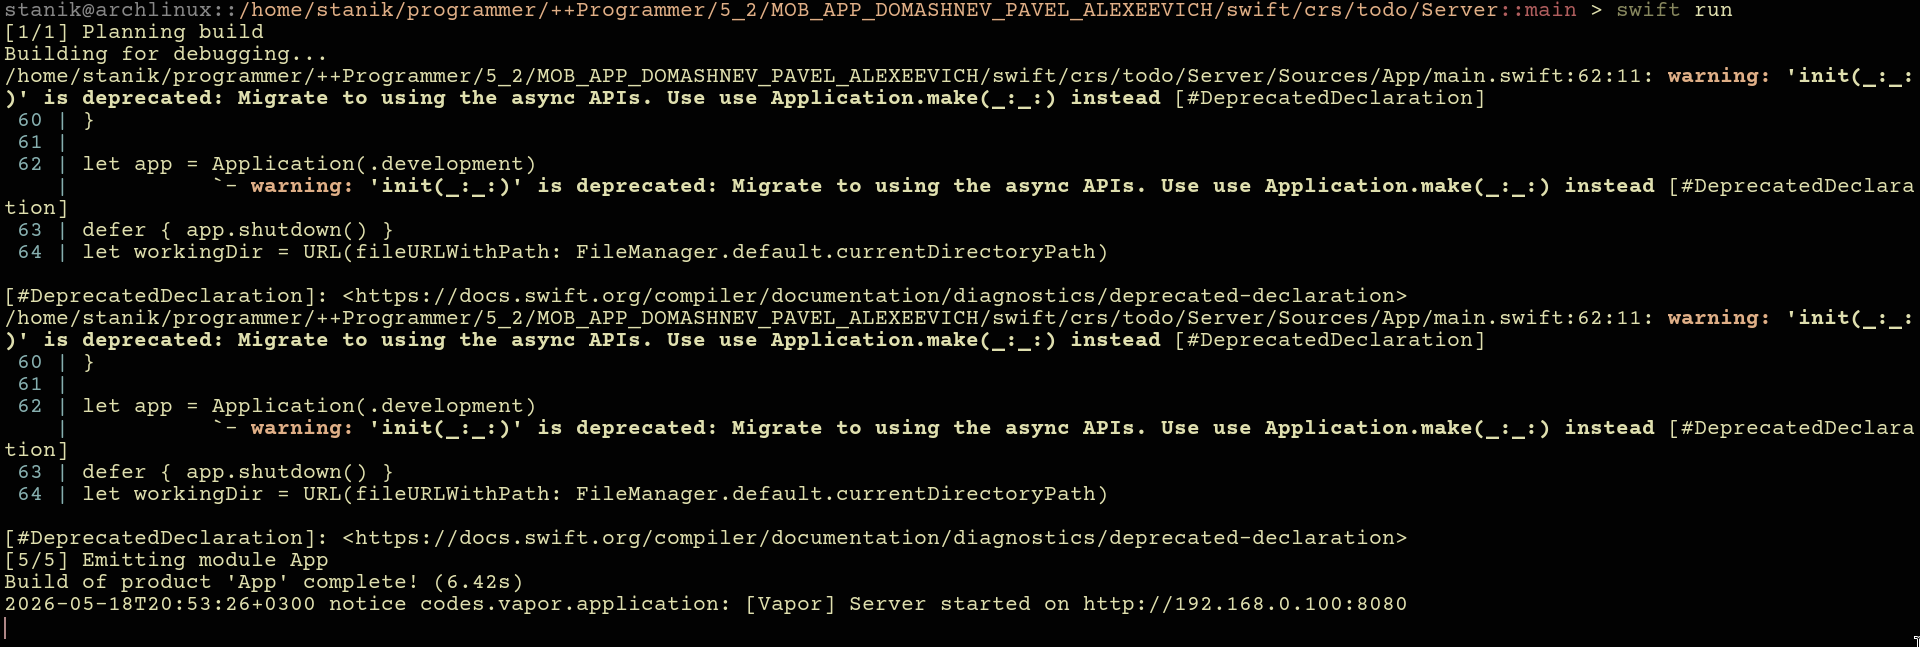
\includegraphics[width=0.78\textwidth]{server.png}
    \refstepcounter{figure}
    \caption*{Рисунок \thefigure\ — Сервер}
    \label{fig:server}
\end{figure}

\newpage

\section{Разработка графического интерфейса клиентского приложения}

\subsection{Назначение графического интерфейса}

Графический интерфейс мобильного приложения предназначен для взаимодействия пользователя с системой управления заметками ``Todo''. Интерфейс обеспечивает создание, просмотр, редактирование, удаление и категоризацию задач, а также предоставляет средства навигации между различными разделами приложения.

Клиентская часть разработана для платформы iOS с использованием фреймворка UIKit. Данный подход позволяет реализовать нативный пользовательский интерфейс, соответствующий требованиям платформы Apple и обеспечивающий высокую производительность приложения.

Основу пользовательского интерфейса составляют экран отображения списка задач, экран категорий, экран просмотра подробной информации о задаче и экран добавления новой задачи.

\subsection{Архитектура графического интерфейса}

Построение пользовательского интерфейса выполнено на основе паттерна навигации \texttt{UINavigationController}, который обеспечивает переход между экранами приложения.

Каждый экран реализован отдельным контроллером представления. Такой подход позволяет изолировать логику отображения и упростить поддержку приложения.

Навигация между экранами осуществляется посредством последовательного перехода между контроллерами, что соответствует типичной архитектуре iOS-приложений.

\subsection{Экран списка задач}

Основным экраном приложения является экран списка задач, реализованный посредством класса \texttt{TasksTableViewController}, наследуемого от \texttt{UITableViewController}.

Данный экран предназначен для отображения списка пользовательских задач и реализует следующие функции:

\begin{itemize}
    \item отображение списка всех задач;
    \item переход к экрану подробной информации;
    \item добавление новой задачи;
    \item удаление существующей задачи;
    \item синхронизация данных с сервером.
\end{itemize}

Для отображения данных используется компонент \texttt{UITableView}. Каждая строка таблицы содержит:

\begin{itemize}
    \item название задачи;
    \item категорию;
    \item состояние выполнения.
\end{itemize}

При выборе строки выполняется переход на экран детальной информации о задаче.

Для добавления новой записи используется системная кнопка \texttt{UIBarButtonItem} с типом \texttt{add}, расположенная в панели навигации. При её выборе открывается экран создания задачи.

Также реализован механизм удаления элементов посредством встроенного режима редактирования таблицы. Удаление задачи приводит к её исключению из локального хранилища и отправке запроса удаления на сервер.

На рисунке 2 представлен экран списка задач клиентского приложения.

\begin{figure}[H]
    \centering
    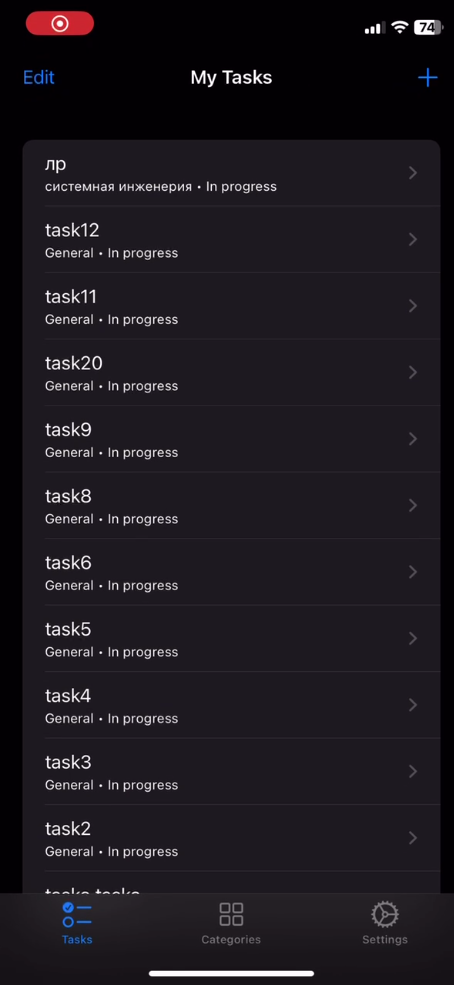
\includegraphics[width=0.78\textwidth]{client.png}
    \refstepcounter{figure}
    \caption*{Рисунок \thefigure\ — Экран списка задач клиентского приложения}
    \label{fig:client}
\end{figure}

\subsection{Экран категорий}

Для представления информации о распределении задач по категориям реализован экран категорий, представленный классом \texttt{CategoriesCollectionViewController}.

Данный экран построен на основе компонента \texttt{UICollectionViewController}, что удовлетворяет требованиям задания кафедры по использованию \texttt{CollectionViewController}.

Экран предназначен для отображения статистической информации о категориях задач. Для каждой категории отображаются:

\begin{itemize}
    \item название категории;
    \item количество задач, относящихся к данной категории.
\end{itemize}

Список категорий формируется автоматически на основе имеющихся пользовательских задач посредством группировки данных.

Для визуального представления используется пользовательская ячейка \texttt{CategoryCell}, содержащая текстовые элементы интерфейса:

\begin{itemize}
    \item название категории;
    \item количество задач.
\end{itemize}

Каждая ячейка имеет скруглённые границы и использует системные стили отображения iOS, что обеспечивает визуальную согласованность интерфейса.

\subsection{Использование Auto Layout}

Построение интерфейса выполнено с использованием технологии Auto Layout и системы ограничений (\texttt{Constraints}).

Для размещения элементов внутри пользовательских ячеек применяются ограничения, задаваемые программным способом посредством \texttt{NSLayoutConstraint}.

Например, элементы интерфейса внутри ячейки категории располагаются при помощи вертикального контейнера \texttt{UIStackView}, а позиционирование осуществляется через ограничения:

\begin{itemize}
    \item выравнивание по левому краю;
    \item выравнивание по правому краю;
    \item центрирование по вертикали.
\end{itemize}

Применение Auto Layout позволяет обеспечить корректное масштабирование интерфейса на устройствах с различными размерами экрана и ориентацией.

\subsection{Организация пользовательских компонентов}

Для отображения информации используются стандартные компоненты UIKit:

\begin{itemize}
    \item \texttt{UITableView} --- отображение списка задач;
    \item \texttt{UICollectionView} --- отображение категорий;
    \item \texttt{UILabel} --- вывод текстовой информации;
    \item \texttt{UIStackView} --- группировка элементов интерфейса;
    \item \texttt{UIBarButtonItem} --- реализация навигационных действий.
\end{itemize}

Использование стандартных компонентов платформы обеспечивает единообразие визуального оформления и соответствие рекомендациям Human Interface Guidelines.

\subsection{Синхронизация интерфейса с данными}

При запуске приложения выполняется загрузка локально сохранённых данных и их отображение в таблице.

После инициализации интерфейса осуществляется асинхронная синхронизация с сервером посредством REST API. Полученные данные сохраняются в локальное хранилище и отображаются пользователю.

При добавлении, изменении или удалении задачи интерфейс обновляется автоматически, что обеспечивает актуальность отображаемой информации.

Для обновления содержимого используются механизмы перезагрузки источников данных компонентов \texttt{UITableView} и \texttt{UICollectionView}.

\subsection{Особенности пользовательского интерфейса}

Разработанный интерфейс обладает следующими особенностями:

\begin{itemize}
    \item использование нативных компонентов iOS;
    \item поддержка навигации между экранами;
    \item отображение списка задач и категорий;
    \item использование адаптивной вёрстки на основе Auto Layout;
    \item поддержка операций создания, удаления и просмотра задач;
    \item автоматическое обновление интерфейса после синхронизации данных.
\end{itemize}

\newpage
\section{Организация работы клиента с локальным и серверным хранилищем данных}

\subsection{Общая схема хранения данных}

Клиентское приложение реализует двухуровневую систему хранения данных, включающую локальное и удалённое хранилище.

Локальное хранение реализовано с использованием базы данных SQLite и предназначено для сохранения пользовательских задач непосредственно на мобильном устройстве. Это обеспечивает возможность доступа к данным без постоянного подключения к сети и ускоряет работу интерфейса.

Удалённое хранение реализовано посредством взаимодействия с серверным REST API, обеспечивающим централизованное хранение и синхронизацию задач.

Таким образом, клиентское приложение использует гибридную модель работы с данными, при которой локальная база обеспечивает быстрый доступ к информации, а серверная часть используется для централизованного хранения и обмена данными.

\subsection{Работа с локальной базой данных}

Для хранения задач на мобильном устройстве используется встроенная система управления базами данных SQLite.

Доступ к локальному хранилищу реализован классом \texttt{SQLiteTaskStore}, который отвечает за:

\begin{itemize}
    \item создание базы данных;
    \item создание таблицы задач;
    \item получение списка задач;
    \item добавление и обновление записей;
    \item удаление задач.
\end{itemize}

Файл базы данных создаётся в каталоге документов приложения (\texttt{Documents}), что обеспечивает сохранение информации между запусками программы.

При инициализации объекта выполняется открытие соединения с базой данных и создание таблицы задач в случае её отсутствия.

\subsection{Структура локальной базы данных}

В локальной базе данных используется таблица \texttt{tasks}, предназначенная для хранения пользовательских задач.

Структура таблицы включает следующие поля:

\begin{table}[H]
\centering
\caption{Структура таблицы \texttt{tasks}}
\label{table:sqlite_tasks}
\begin{tabular}{|p{4cm}|p{3cm}|p{6cm}|}
\hline
\textbf{Поле} & \textbf{Тип} & \textbf{Назначение} \\
\hline
\texttt{id} & TEXT & Уникальный идентификатор задачи \\
\hline
\texttt{title} & TEXT & Название задачи \\
\hline
\texttt{notes} & TEXT & Текстовое описание \\
\hline
\texttt{is\_done} & INTEGER & Статус выполнения задачи \\
\hline
\texttt{category} & TEXT & Категория задачи \\
\hline
\texttt{updated\_at} & TEXT & Время последнего изменения \\
\hline
\end{tabular}
\end{table}

Поле \texttt{id} используется как первичный ключ таблицы, что гарантирует уникальность каждой записи.

Для хранения даты изменения используется строковое представление времени в формате ISO 8601. Такой подход обеспечивает совместимость при обмене данными между клиентом и сервером.

\subsection{Операции над локальными данными}

Работа с локальной базой данных осуществляется посредством SQL-запросов.

Получение списка задач выполняется с помощью запроса выборки:

\begin{itemize}
    \item чтение записей из таблицы;
    \item сортировка по времени обновления;
    \item преобразование результатов в объекты приложения.
\end{itemize}

Добавление и обновление задач выполняется посредством операции \texttt{INSERT OR REPLACE}. Такой механизм позволяет использовать единый алгоритм как для создания новой записи, так и для изменения существующей.

Удаление задачи выполняется SQL-запросом \texttt{DELETE}, принимающим идентификатор задачи.

После выполнения SQL-запросов информация немедленно становится доступной пользовательскому интерфейсу, что позволяет обеспечить актуальное отображение данных.

\subsection{Взаимодействие с серверным хранилищем}

Обмен данными с сервером реализован отдельным компонентом \texttt{APIClient}, который отвечает за выполнение HTTP-запросов к REST API.

Для сетевого взаимодействия используется \texttt{URLSession}, входящий в состав платформы iOS.

Компонент поддерживает следующие операции:

\begin{itemize}
    \item получение списка задач с сервера;
    \item добавление или обновление задачи;
    \item удаление задачи.
\end{itemize}

Все операции выполняются асинхронно, что предотвращает блокировку пользовательского интерфейса при ожидании ответа сервера.

\subsection{Получение данных с сервера}

Получение списка задач осуществляется посредством HTTP-запроса метода \texttt{GET} к маршруту:

\begin{center}
\texttt{/tasks}
\end{center}

После получения ответа выполняется:

\begin{itemize}
    \item проверка HTTP-кода состояния;
    \item декодирование JSON-документа;
    \item преобразование полученных данных в объекты приложения.
\end{itemize}

Для обработки даты используется формат ISO 8601, что обеспечивает единое представление времени как на сервере, так и на клиенте.

Полученные задачи сохраняются в локальную базу данных и становятся доступными для отображения в пользовательском интерфейсе.

\subsection{Добавление и изменение задач на сервере}

Для сохранения задачи на сервере используется HTTP-метод \texttt{POST}.

Клиент сериализует объект задачи в JSON-документ и передаёт его серверу вместе с HTTP-запросом.

Запрос включает заголовок:

\begin{center}
\texttt{Content-Type: application/json}
\end{center}

После успешного выполнения операции сервер возвращает код состояния \texttt{201 Created}, подтверждающий сохранение объекта.

При изменении задачи используется тот же механизм, поскольку серверная часть реализует объединённую операцию добавления и обновления.

\subsection{Удаление данных с сервера}

Удаление задачи выполняется посредством HTTP-запроса метода \texttt{DELETE}.

В адресе запроса передаётся уникальный идентификатор задачи.

После успешного удаления сервер возвращает код состояния:

\begin{center}
\texttt{204 No Content}
\end{center}

Если задача отсутствует на сервере, используется код:

\begin{center}
\texttt{404 Not Found}
\end{center}

Подобный подход позволяет клиентскому приложению корректно обрабатывать ситуации рассинхронизации данных.

\subsection{Механизм синхронизации данных}

При запуске приложения сначала загружаются данные из локальной базы SQLite, после чего выполняется асинхронный запрос к серверу.

Данный подход обеспечивает быстрое отображение информации пользователю даже при нестабильном интернет-соединении.

Алгоритм синхронизации можно представить следующим образом:

\begin{enumerate}
    \item загрузка данных из SQLite;
    \item отображение задач в интерфейсе;
    \item выполнение запроса к REST API;
    \item получение актуальных данных с сервера;
    \item сохранение данных в локальную базу;
    \item обновление пользовательского интерфейса.
\end{enumerate}

При добавлении, редактировании или удалении задачи изменения сначала сохраняются локально, после чего асинхронно отправляются на сервер.

Такой подход позволяет минимизировать задержки пользовательского интерфейса и обеспечивает возможность частичной работы приложения при отсутствии сети.

\newpage
\section{Список источников}

\begin{enumerate}
\item Apple Developer Documentation: UIKit [Электронный ресурс] /
Режим доступа: https://developer.apple.com/documentation/uikit/,
свободный — 18.05.2026.

\item Apple Developer Documentation: URLSession [Электронный ресурс] /
Режим доступа: https://developer.apple.com/documentation/foundation/urlsession/,
свободный — 18.05.2026.

\item Apple Developer Documentation: SQLite3 API [Электронный ресурс] /
Режим доступа: https://developer.apple.com/library/archive/documentation/General/Reference/SQLLiteCRef/,
свободный — 18.05.2026.

\item Vapor Framework Documentation [Электронный ресурс] /
Режим доступа: https://docs.vapor.codes/,
свободный — 18.05.2026.

\item SQLite Documentation [Электронный ресурс] /
Режим доступа: https://www.sqlite.org/docs.html,
свободный — 18.05.2026.
\end{enumerate}
\newpage

\section{Вывод}

В ходе выполнения курсового проекта было разработано мобильное приложение ``Todo'' для платформы iOS, предназначенное для создания, хранения и управления пользовательскими задачами.

В процессе разработки была спроектирована и реализована серверная часть приложения, предоставляющая REST API для централизованного хранения данных. Сервер обеспечивает выполнение основных операций над задачами, включая создание, получение, обновление и удаление записей, а также поддерживает обмен данными в формате JSON.

Была реализована клиентская часть приложения с использованием средств платформы iOS и фреймворка UIKit. Разработанный графический интерфейс включает экран списка задач, экран категорий и дополнительные средства взаимодействия с пользовательскими данными. При проектировании интерфейса использовались стандартные компоненты платформы, включая \texttt{UITableViewController} и \texttt{UICollectionViewController}, а построение интерфейса выполнено с применением Auto Layout и системы ограничений.

Для хранения информации на мобильном устройстве реализована локальная база данных SQLite, обеспечивающая сохранность данных между запусками приложения и возможность быстрого доступа к ним. Дополнительно реализовано взаимодействие с удалённым серверным хранилищем посредством REST API, что позволило организовать синхронизацию данных между клиентом и сервером.

В рамках проекта были реализованы механизмы асинхронной обработки сетевых запросов, сериализации данных и обновления пользовательского интерфейса после изменения состояния хранилища.

В результате выполнения работы были выполнены основные требования, предъявляемые к курсовому проекту: реализовано мобильное приложение для iOS, разработан собственный сервер с REST API, использована локальная база данных SQLite, применены \texttt{TableViewController} и \texttt{CollectionViewController}, реализована адаптивная вёрстка с использованием Auto Layout и обеспечено централизованное хранение пользовательских данных.

Поставленная цель разработки мобильного приложения для управления задачами была достигнута.

\end{document}
